\documentclass[]{ximera}
%handout:  for handout version with no solutions or instructor notes
%handout,instructornotes:  for instructor version with just problems and notes, no solutions
%noinstructornotes:  shows only problem and solutions

%% handout
%% space
%% newpage
%% numbers
%% nooutcomes

%I added the commands here so that I would't have to keep looking them up
%\newcommand{\RR}{\mathbb R}
%\renewcommand{\d}{\,d}
%\newcommand{\dd}[2][]{\frac{d #1}{d #2}}
%\renewcommand{\l}{\ell}
%\newcommand{\ddx}{\frac{d}{dx}}
%\everymath{\displaystyle}
%\newcommand{\dfn}{\textbf}
%\newcommand{\eval}[1]{\bigg[ #1 \bigg]}

%\begin{image}
%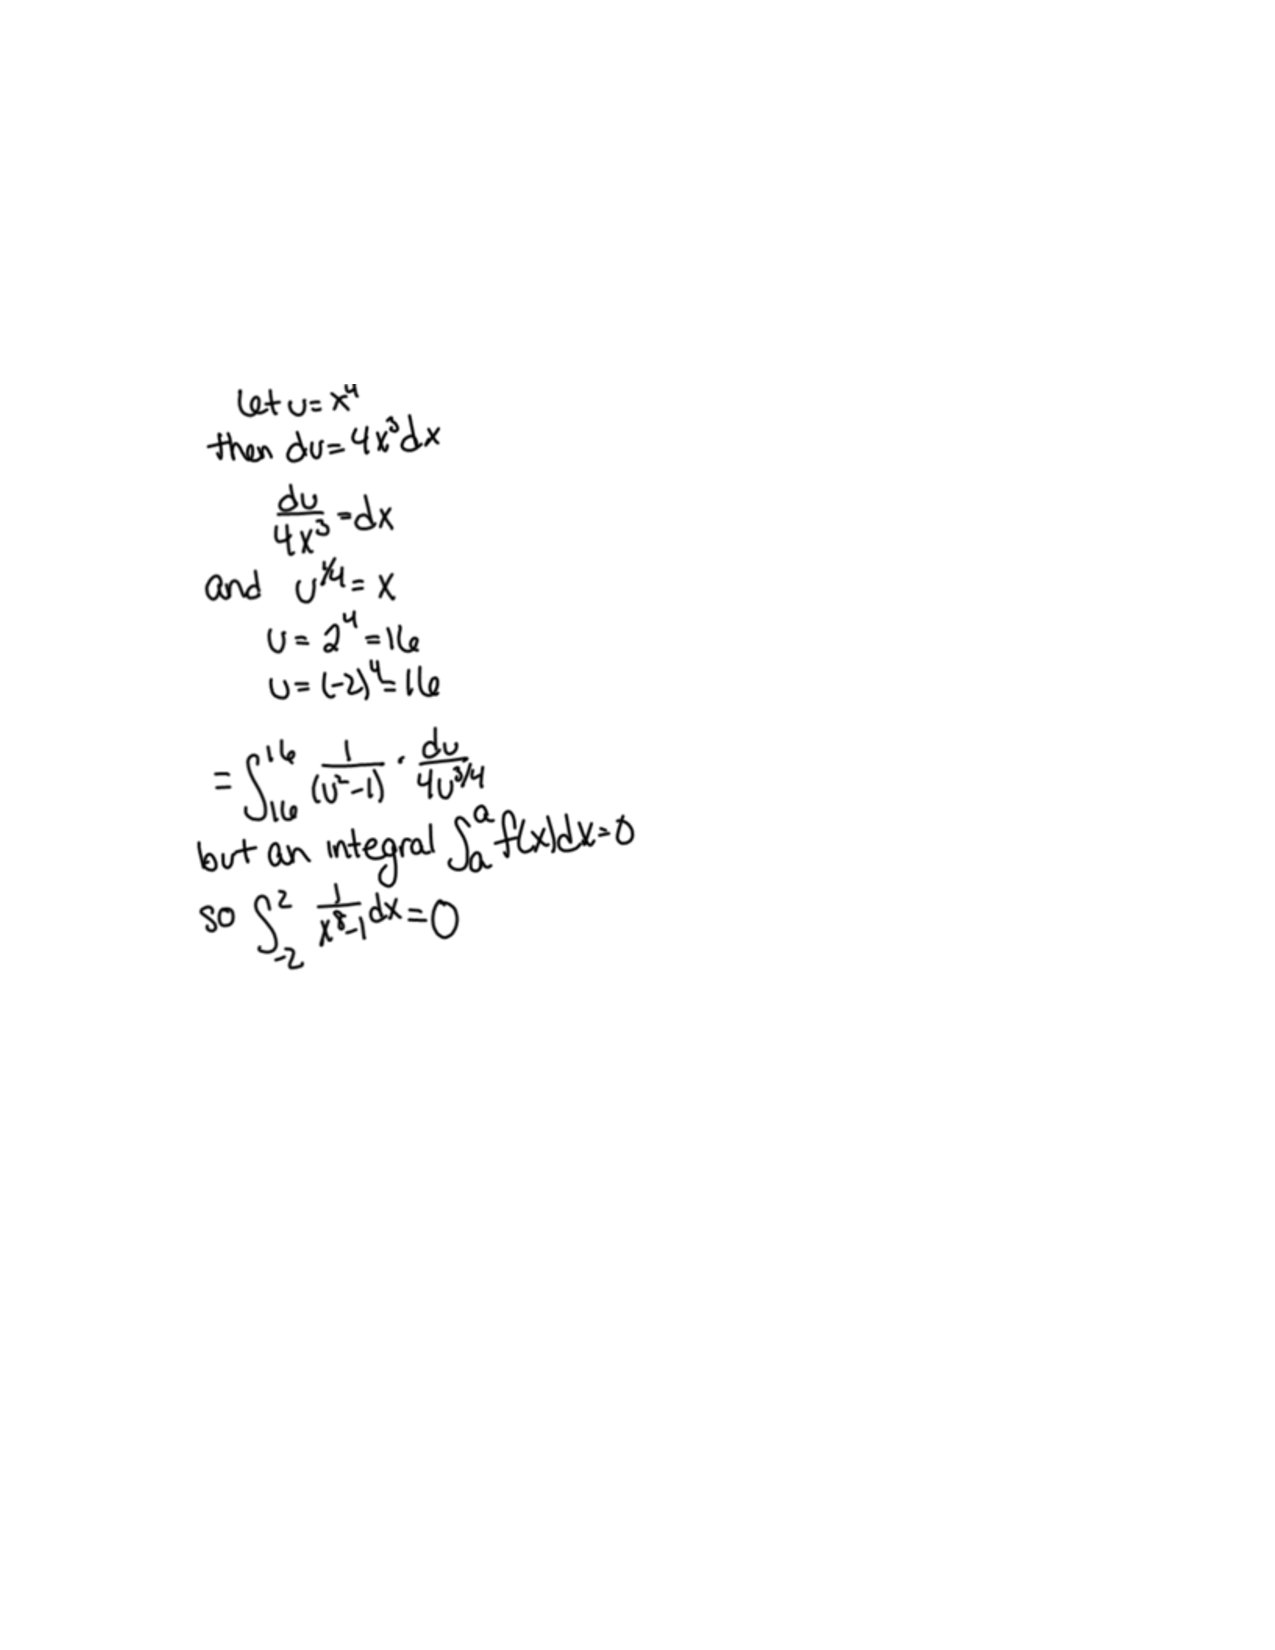
\includegraphics[trim= 170 420 250 180]{Figure1.pdf}
%\end{image}

%add a ``.'' below when used in a specific directory.
\newcommand{\RR}{\mathbb R}
\renewcommand{\d}{\,d}
\newcommand{\dd}[2][]{\frac{d #1}{d #2}}
\renewcommand{\l}{\ell}
\newcommand{\ddx}{\frac{d}{dx}}
\newcommand{\dfn}{\textbf}
\newcommand{\eval}[1]{\bigg[ #1 \bigg]}

\usepackage{multicol}

\renewenvironment{freeResponse}{
\ifhandout\setbox0\vbox\bgroup\else
\begin{trivlist}\item[\hskip \labelsep\bfseries Solution:\hspace{2ex}]
\fi}
{\ifhandout\egroup\else
\end{trivlist}
\fi} %% we can turn off input when making a master document

\title{Improper integrals}  

\begin{document}
\begin{abstract}		\end{abstract}
\maketitle



\section{Warm up:}
True or False:  It is possible for a region to be infinitely long but have a finite area.
	\begin{freeResponse}
	True.  Consider the region below the curve $y=\frac{1}{x^2}$, $x \geq 1$.
	\end{freeResponse}
	
\begin{instructorNotes}

\end{instructorNotes}








\section{Group work:}



%problem 1
\begin{problem}
Review of limits:
	\begin{enumerate}
	
	\item  $\lim_{x \to -\infty} \left( 3x^{-6} + e^{5x} + \frac{\sin x}{x^2 + 3} \right)$
	\begin{freeResponse}
	Recall that the limit of a sum is the sum of the limits, provided that those limits exist.
		\begin{itemize}
		\item  $\lim_{x \to -\infty} 3x^{-6} = \lim_{x \to -\infty} \frac{3}{x^6} = 0$.
		\item  $\lim_{x \to -\infty} e^{5x} = 0$.
		\item  $\lim_{x \to -\infty} \frac{\sin x}{x^2 + 3} = 0$  
		
		\vspace{8pt}
		
		{\color{red} \text{To rigorously prove this, you need to use the squeeze theorem.}}
		\end{itemize}
	Thus, 
		\[
		\lim_{x \to -\infty} \left( 3x^{-6} + e^{5x} + \frac{\sin x}{x^2 + 3} \right) = 0
		\]
	\end{freeResponse}
	
	
	
	\item  $\lim_{x \to \infty} \frac{x}{\sqrt{9x^2+4}}$
	\begin{freeResponse}
		\begin{align*}
		\lim_{x \to \infty} \frac{x}{\sqrt{9x^2+4}}
		&= \lim_{x \to \infty} \frac{x}{\sqrt{x^2} \cdot {\sqrt{9 + \frac{4}{x^2}}}}  \\
		&= \lim_{x \to \infty} \frac{x}{|x| \cdot \sqrt{9 + \frac{4}{x^2}}}  \\
		&= \lim_{x \to \infty} \frac{x}{x \cdot \sqrt{9 + \frac{4}{x^2}}}  \\
		&= \lim_{x \to \infty} \frac{1}{\sqrt{9 + \frac{4}{x^2}}}  \\
		&= \frac{1}{\sqrt{9 + 0}} = \frac{1}{3}.
		\end{align*}
	\end{freeResponse}
	
	
	
	\item  $\lim_{x \to -\infty} \arctan x$
	\begin{freeResponse}
	$\lim_{x \to -\infty} \arctan x = - \frac{\pi}{2}. $
	\end{freeResponse}
	
	\end{enumerate}
		
\end{problem}

\begin{instructorNotes}

\end{instructorNotes}








%problem 2
\begin{problem}
In each of the following, determine if the given integral converges or diverges.  
If it converges, find the value.

	\begin{enumerate}
	
	\item  $\int_{-1}^{\infty} \frac{3}{2x+1} \d x$
	\begin{freeResponse}
	The function $\frac{3}{2x+1}$ has a vertical asymptote at $x=- \frac{1}{2}$.  
	So we rewrite the original integral as
		\[
		\int_{-1}^{\infty} \frac{3}{2x+1} \d x = \lim_{a \to -\frac{1}{2}^-} \int_{-1}^a \frac{3}{2x+1} \d x  
		+ \lim_{b \to -\frac{1}{2}^+} \int_b^0 \frac{3}{2x+1} \d x + \lim_{c \to \infty} \int_0^c \frac{3}{2x+1} \d x.
		\]
	The latter integral does not exist.  
	To see this, just note that
		\begin{align*}
		 \lim_{c \to \infty} \int_0^c \frac{3}{2x+1} \d x 
		 &= \lim_{c \to \infty} \eval{\frac{3}{2} \ln|2x+1|}_0^c  \\
		 &= \lim_{c \to \infty} \frac{3}{2} \ln|2c+1| = \infty.
		\end{align*}
	Therefore, 
		\[
		\int_{-1}^{\infty} \frac{3}{2x+1} \d x \; \text{ diverges.}
		\]
	\end{freeResponse}
	
	
	
	\item  $\int_{-\infty}^{\infty} x e^{-x} \d x$
	\begin{freeResponse}
	\[
	\int_{-\infty}^{\infty} x e^{-x} \d x = \lim_{a \to -\infty} \int_a^0 xe^{-x} \d x + \lim_{b \to \infty} \int_0^b xe^{-x} \d x.
	\]
	The first of these integrals does not exist.  
	To see this, we apply integration by parts
		\begin{align*}
		\lim_{a \to -\infty} \int_a^0 xe^{-x} \d x
		&= \lim_{a \to -\infty} \left( \eval{-xe^{-x}}_a^0 + \int_a^0 e^{-x} \d x \right)  \\
		&= \lim_{a \to -\infty} \left( \left[ 0 + ae^{-a} \right] + \eval{-e^{-x}}_a^0 \right)  \\
		&= \lim_{a \to -\infty} \left( ae^{-a} + e^{-a} - 1 \right)  \\
		&= \lim_{a \to -\infty} \left( e^{-a}(a+1) - 1 \right)  \\
		&= - \infty.
		\end{align*}
	Thus
		\[
		\int_{-\infty}^{\infty} x e^{-x} \d x \; \text{ diverges.}
		\]
	\end{freeResponse}
	
	
	
	\item  $\int_6^{\infty} \frac{2-4x}{2x^2 - 13x + 20} \d x$
	\begin{freeResponse}
	First notice that we can factor the denominator as
		\[
		2x^2 - 13x + 20 = (2x-5)(x-4).
		\]
	So we find a partial fraction decomposition of the integrand
		\[
		\frac{2-4x}{(2x-5)(x-4)} = \frac{A}{2x-5} + \frac{B}{x-4}
		\]
	\end{freeResponse}
	
	\end{enumerate}
	
\end{problem}

\begin{instructorNotes}
Make sure that students write in the limit notation throughout their work, with the limit taken after the definite integral has been evaluated.
	\begin{enumerate}
	\item has a vertical asymptote as well as a limit going to infinity.
	\item is by parts, and L'Hospital's Rule will be useful for the limit.
	\item will need partial fractions.  
	The coefficients of the decomposition are rigged to be opposites of each other, so that one can use properties of logarithms to aid in taking the limit.
	\end{enumerate}
\end{instructorNotes}







%problem 3
\begin{problem}
Find the volume of the solid whose base is the region where $x \geq 1$, $y \geq 0$, and below the curve $y=\frac{1}{x^4}$, and whose cross sections perpendicular to the $x$-axis are squares.
	\begin{freeResponse}
	
	\end{freeResponse}

\end{problem}

\begin{instructorNotes}

\end{instructorNotes}

















	
	
	
	
	
	
	
	
	

	










								
				
				
	














\end{document} 


















